\subsection{Présentation de l'approche composant}
    
Le terme de «~composant~», définit dans l'approche de l'ingénierie du logiciel basée sur les composants (\emph{Component-Based Software Engineering -- CBSE}) étant très générique, en donner une définition exacte et précise paraît difficile car dépend fortement du contexte de son utilisation. Cependant on peut se baser sur des définitions faites dans la littérature :

\begin{quote}
  \emph{ A software component is a unit of composition with contractually specified interfaces and explicit context dependencies only. A software component can be deployed independently and is subject to composition by third parties.} \cite{Szyperski:2002:CSB:515228}
\end{quote}
  
\begin{quote}
  \emph{ A component is a nontrivial, nearly independent, and replaceable part of a system that fulfills a clear function in the context of a well-defined architecture. A component conforms to and provides the physical realization of a set of interfaces.} \cite{kruchten1998modeling}
\end{quote}
  
\begin{quote}
  \emph{ A component is a unit of distributed program structure that encapsulates its implementation behind a strict interface comprised of services provided by the component to other components in the system and services required by the component and implemented elsewhere. The explicit declaration of a component's requirements increases reuse by decoupling components from their operating environment.} \cite{pryce1998component}
\end{quote}
  
Ces différentes définitions permettent de faire ressortir des notions qui se retrouvent dans la plupart des approches à composants : 
    
\begin{description}

  \item[composition] Le mécanisme de composition permet de créer à partir d'un assemblage de << connexion >> de composants, un nouveau composant plus complexe, en encapsulant des composants afin de pouvoir réutiliser directement cette assemblage. Ce nouveau composant est dit composite car composé de composants qui deviennent des sous-composants (composants interne), pouvant être eux aussi des composants composites ou des composants primitifs \footnote{un composant est dit primitif s'il ne contient pas de sous-composants}.
  
  \item[interfaces] C. Szyperski définit une interface d'un composant comme étant un point d'accès au service du composant \cite{szyperski1999components} permettant de décrire comment peuvent être assemblés nos composants ou utilisés dans notre architecture. On parle d'interfaces << requises >>, pour celles qui permettent de décrire les besoins d'un composant et d'interfaces << fournies >>, les interfaces permettant de définir les fonctionnalités que proposent notre composant aux autres composants.
  
  \item[architecture] La notion d'architecture permet de représenter le plan de notre application et permet de décrire comment doit être conçu notre application afin de respecter les spécifications mises en place.
 
  \item[service] Les services permettent de représenter la logique métier d'un composant. Géné\-ralement présent uniquement dans des composants primitifs, certaines approches essaient de définir des services pour des composants composites. 
  
  \item[indépendance] Il faut voir un composant comme un élément indépendant de tous systèmes. Il doit être assez générique pour pouvoir se connecter à d'autres composants au sein d'une nouvelle application en fournissant un ensemble de services, sens être trop spécifique à un système afin de répondre à un besoin précis.
  
\end{description}
    
    
\subsection{Les principes de l'approche à composant}

  De nombreux concepts permettent la notion de réutilisabilité pour le développement (appel de fonction, importation de module, héritage entre classe, paramétrage de framework, assemblage de composants, etc.). Cependant même si ses différentes techniques permettant de mettre en avant cette notion de réutilisabilité, les composants on fait de la réutilisation le fer de lance de leurs approches.\\\par  
    
  On identifie deux nouveaux acteurs de l'approche à composants \cite{fabresse2007decoupage} : le dévelop\-peur de composants et l’architecte d’application (cf figure \ref{fig:reusecomponent}). Le rôle du développeur va consister à réaliser des composants indépendants. Quant à l'architecte, il récupère les composants déjà créés par un développeur et réalise une intégration dans son assemblage de composants existant. Il est bien sûr possible pour une personne d'avoir les deux casquettes, mais il doit rendre son composant indépendant de l'application. \\\par 
      
\begin{figure}[!t]
\centering
\scalebox{.5}{
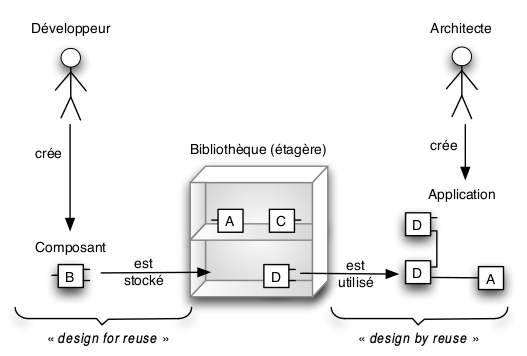
\includegraphics{images/reuse.png}
}
\caption{Vision simplifiée du processus de développement par composants, extrait de \cite{fabresse2007decoupage}}
\label{fig:reusecomponent}
\end{figure}
  
  Nous avons vue que l'architecture logiciel permettait de définir comment notre application devait être construite. C'est pour cela que nous avons besoin de visibilité sur cette architecture afin de bien appréhender comment notre application est réalisée et de visualiser toute les interactions entre les éléments de l'application, permettant ainsi de vérifier que cette architecture respecte bien les spécifications. Dans le monde objet, la notion d'architecture est réalisé lors de la phase de conception de l'application et même si le développeur peut s'aider d'outil de représentation graphique, comme UML, cette représentation n'est que peu maintenue lors de la phase d'implémentation, ce qui ne permet plus de voir les modifications apportées par celle-ci et donc n'assure plus que cette nouvelle architecture soit conforme aux spécifications. \\\par
  
  Le monde des composants arrive à corriger cela, en rendant explicite cette visibilité sur l'architecture, soit à la manière des ADLs (Architecture Description Languages), qui permettent de décrire la structure et de définir le comportement des composants à travers leurs assemblages, par une représentation abstraite, soit directement dans l'implémentation des composants par l'approche des langages à composants, qui définissent l'architecture au sein même des composants. Par conséquent, même si pendant la phase d'implémentation on décide de modifier l'architecture de nos composants, on ne perdra pas la visibilité sur l'architecture de notre application car elle est écrite explicitement. \\\par
  
\subsection{Les grandes approches du développement à base de composants}
      
      \subsubsection{La famille des génératives}
      
      La famille des génératives se situe à un haut niveau d'abstraction afin de modéliser et gérer des systèmes logiciels complexes. Cette représentation se base généralement sur les ADLs, permettant de décrire les architectures logiciels à base de composants en y décrivant leurs comportements, leurs interactions avec les autres composants et leurs configurations ainsi que leurs besoins explicites. La stratégie de cette approche générative consiste donc dans la modélisation d'une architecture de composants << initial >> décrite de manière formelle afin de générer un << squelette >> d'application dans un langage de programmation précis qui respectera les spécifications du système. Cette représentation étant abstraite, elle est indépendante des langages de programmation qui implémente les composants, permettant ainsi de s'adapter à tous types de plateforme. \\\par
      
          \textbf{UML -- un langage de modélisation graphique pour composants}
      
      UML (Unified Modeling Language) est un langage de modélisation graphique standardisé par l'OMG (\emph{Objet management groupe}) \footnote{http://www.omg.org/spec/UML}. Dans sa première version, UML intègre déjà la notion de composant, comme étant une entité indépendante et communiquant avec d'autres composants au travers d'interfaces. La version 2.0 d'UML \cite{specificationuml} a permis d'améliorer cette vision des composants, en s'inspirant aussi des mécanismes et concepts des ADLs, introduisant la notion de port, de connecteur et de composant composite.

Un composant UML est donc une entité autonome, qui communiquent avec les autres composants de l'architecture au travers d'interfaces, regroupées dans des ports qui expriment des rôles. Un composant peut disposer de plusieurs ports, où un port regroupe un ensemble d'interfaces requises ou fournies. Le port permet donc de réaliser une communication entre l'environnement extérieur du composant et son architecture interne. 
      
 Cette connexion entre composants est permise par la notion de connecteur, qui permet de représenter les possibilités de communication entre les composants. Il existe deux types de connecteurs : d’assemblage et de délégation. Un connecteur d'assemblage permet de lier deux interfaces de deux composants. Avec une interface requise pour notre premier composant et une interface fournie pour notre deuxième composant. Cette connexion ne peut se faire que si les deux interfaces ont la même signature. Un connecteur de délégation quant à lui est utilisé afin de réaliser une connexion entre ses interfaces ou ports vers les interfaces ou ports de ses composants internes, permettant ainsi un délégation d'un besoin ou d'un service vers un composant interne.
        
    UML apporte cet aspect visuel à la représentation des architectures composantes qui manquent aux autres approches, aidant ainsi un architecte à mieux visualiser l'architecture qu'il est en train de construire, mais ne permet pas de réaliser l'implémentation et la manipulation de composants sans le coupler à une autre technique. \\\par 
    
        \textbf{Fractal -- un framework orienté composants intégrant un ADL}
        
        Fractal \cite{bruneton2006fractal} est une spécification d'un modèle à composant proposé par le consortium \emph{ObjectWeb} en 2002, proposant ainsi un framework pour la création d'applications déployables sur un serveur et proposant la création et la manipulation de composant, intégrant aussi un ADL pour la description de l'architecture des composants. Il met en avant le concept de composant composite, de composant partagé, un mécanisme d'introspection et la possibilité de configuration dynamique. 
        
        Un composant Fractal est composé de deux partie, la partie \emph{contenu} qui va contenir les fonctionnalités que propose le composant, en étant soit un composant primitif qui dans son \emph{contenu} va implémenter la logique métier, soit un composant composite qui encapsule un assemblage de composants qui réalise les fonctionnalités attendues. La deuxième partie d'un composant est appelé la \emph{membrane}, qui contient les parties non-fonctionnelles du composant, intégrant les différentes interfaces qui communique avec le monde extérieur, ainsi que les interfaces qui permettent le contrôle du composant.
        
        Une interface a deux type de visibilité : externe qui est visible depuis l’extérieur du composant et permettra une liaison avec d'autre composant et interne permettant une liaison avec son contenu. Une interface peut être de différents rôles, serveur qui est une interface fournie proposant les différents services du composants, cliente qui est une interface requise représentant les besoins du composants et contrôle permettant la configuration dynamique du composants avec la possibilité de modifier ces liaisons avec les composants externe, de modifier son assemblage interne (modification des liaisons internes) et la gestion du cycle de vie du composant.
        
        Afin de pouvoir connecter deux composants entre eux, il faut connecter une interface de l'un avec une interface de l'autre, cette connexion est appelée liaison (\emph{binding}) et peut être de trois types : une liaison normale (\emph{normal binding}) entre une interface serveur externe d'un composant et une interface cliente externe d'un autre composant, une liaison d'export (\emph{export binding}) entre une interface cliente d'un composite et un interface serveur d'un composant interne permettant la délégation d'un service fourni par notre composant composite qui sera fourni par son composant interne, et une liaison d'import (\emph{(import binding}) entre une interface serveur interne d'un composant composite et une interface cliente externe d'un composant interne permettant la délégation d'un besoin de notre composant interne au composant composite.
        
        Étant un modèle abstrait, il permet de s'abstraire de tous langages et de plateformes pour la gestion de composants, dont différentes implémentations ont été réalisées (par exemple en Java avec Julia ou en C++ avec Cecilia). En effet l'ADL qu’intègre Fractal est décrit dans une syntaxe XML et spécifié de manière indépendante des langages de programmation. Les différentes implémentation proposent cependant un mécanisme de génération de code à partir de l'ADL pour réaliser l'implémentation des composants. \\\par

    \subsubsection{La famille des frameworks}     
   
    La famille des frameworks à composants utilise les langages de programmation objets pour la création et la manipulation de composants afin de modéliser un système. Cette approche permet au développeur d'utiliser les composants afin de bien séparer les besoins fonctionnels et les besoins non-fonctionnels. Principalement utilisé dans le monde professionnel, les frameworks à composants proposent aux développeurs de créer, déployer et configurer une application.  \\\par
    
    \textbf{Enterprise JavaBeans -- un framework orienté composants pour la création d'applications distribuées} 
    
    L'approche de composant mise en place par Enterprise JavaBeans (EJB), développée au sein de la plateforme Java Enterprise Edition (JEE), propose un modèle à composants serveur permettant la réalisation d'applications distribuées \cite{specificationejb}.
    
    Un composant EJB s’exécute dans un conteneur au sein d'un serveur JEE. Les conteneurs gèrent les instances des EJB, tandis que le serveur fourni aux conteneurs des besoins non-fonctionnels.
    
    Un composants EJB est regroupé en trois catégories : session, entité et message. Une instance d'un composant entité permet de représenter un concept métier, ayant pour but de représenter des données pouvant être stockées dans une base de données. Une instance d'un composant message permet la gestion de messages asynchrones reçu par le serveur depuis le client. Une instance d'un composant session permet de fournir des services définis par des méthodes, pouvant être sans état (stateless) ou avec état (stateful).
    
    Un composant EJB communique ses services par une interface \emph{remote}, spécifiant ainsi les méthodes que fournit une instance d'un EJB au monde extérieur. Il permet sa configuration et la gestion de son cycle de vie par une interface \emph{home} qui est fournie par son conteneur. Cependant on ne peut définir le besoin d'un EJB au moyen d'une interface requise mais les propriétés d'un EJB sont définies dans un descripteur de déploiement permettant au conteneur EJB de savoir comment gérer les composants pendant leur exécution.
    
    L’approche des EJB ne permet pas la réalisation de composant composite. Ainsi une architecture sera dite << à plats >>, chaque composants seront au même niveau, permettant une vision horizontale de l'architecture, mais cela peut s’avérer répétitif de réaliser l'ensemble de toutes les différentes connexions entre composants sans pouvoir utiliser la composition pour réutiliser un assemblage de composants.
         
    \subsubsection{La famille des langages orientés composants}
    
    \label{sec:presentcomponent}
    
    L'approche des langages orientés composants s'articule autour d'un seul langage de programmation pour permettre de définir une architecture de composants et l'implémen\-ta\-tion de ses composants. Ce regroupement de ses deux principes permet une meilleure facilité de développement, le rendant plus naturel car le programmeur ne doit connaître qu'un seul langage de programmation. Elle permet de résoudre les problèmes que pouvaient avoir les ADLs lors de l'implémentation de leur composants, qui pouvaient ne plus respecter les contraintes architecturales en communicant avec d'autres composants de l'application sans être décrites au niveau de l'architecture mais au sein du code source. \\\par 
    
      \textbf{ArchJava -- un langage orienté composants} 
      
      ArchJava \footnote{http://www.archjava.org/} créé en 2001 \cite{aldrich2002archjava}, s'inspire de l'approche composant que proposent les ADLs pour la description d'architecture, tout en permettant l'implémentation de ces composants au sein d'un nouveau langage qui est une extension du langage Java.
      
      Un composant est dans ce monde un <<objet particulier>>, qui s'obtient par instanciation de la classe \texttt{component class}. Cette classe de composant permet de regrouper les informations du composants : ses ports, ses méthodes, ses attributs et permet aussi de décrire son assemblage interne à travers des connexions.
      
  Deux composants ne peuvent communiquer entre eux que s'ils sont explicitement connectés par la primitive \texttt{connect}. Cette primitive introduit pour la première fois dans l'histoire des approches à composant la connexion entre composants par la liaison de leurs ports respectifs. 
  
 Un port définit une liste de méthodes fournies et requises, différenciées respectivement par les primitives \texttt{provides} et \texttt{requires}. Une méthode fournie permet d'introduire une fonctionnalité proposée par le composant au monde extérieur. Les autres composants n'ont accès à cette méthode que par le biais du port. Une méthode requise, quant à elle permet de décrire une fonctionnalité attendue par notre composant. Deux ports ne peuvent se lier entre eux que si les signatures des méthodes requises et fournies qu'ils définissent sont compatibles entre eux.  
      
Une classe de composant peut hériter de toutes les propriétés de la super-classe composant dont elle hérite, que ce soit les méthodes, les ports ou connexions, et permet d'en introduire de nouvelles. On peut redéfinir des méthodes fournies, mais l'ajout de ports ne peut introduire que des méthodes fournies.

  ArchJava offre la compatibilité avec les architectures logiciels Java, au sens où une classe de composant peut hériter d'une classe Java << classique >>. Cependant les contraintes architecturales ne sont plus garanties par ArchJava. Deux composants ne peuvent se passer une référence vers un autre composant, afin de réaliser un transfert de données, toutefois les composants peuvent s'échanger une référence vers un objet, ce qui ne permet plus de visualiser l'architecture logiciel. Un programmeur en ArchJava devra toujours ce demander s'il vaut mieux créer un composant ou un objet pour réaliser une nouvelle fonctionnalité.

         


    
      
